La búsqueda binaria es un algoritmo en que se utilizan operaciones lógicas como AND y OR con el fin de encontrar documentos que contienen los términos solicitados en la consulta, asumiendo que ello indica que son relevantes para dicha necesidad de información. Para llevar a cabo la búsqueda de manera eficiente, se crea una matriz binaria indicando los términos que contiene cada documento, dando a la técnica el nombre de \textit{búsqueda binaria}. A continuación, se explica detalladamente el proceso que sigue la técnica.

\subsubsection{Matriz binaria}
Una vez se conoce de cada documento los términos que contiene y su frecuencia, se procede a construir la matriz binaria. Las filas de esta matriz corresponden a los documentos que se consideran en la búsqueda y las filas corresponden a los términos existentes en el diccionario. Siendo así, los registros de cada columna que corresponden a uno indican que ese término existe en el documento indicado por la columna. Cabe resaltar que la frecuencia no es considerada en esta técnica. En la figura \ref{fig:b_matrix} se muestra un ejemplo de cómo se vería una matriz binaria.\\

\begin{figure}[H]
    \centering
    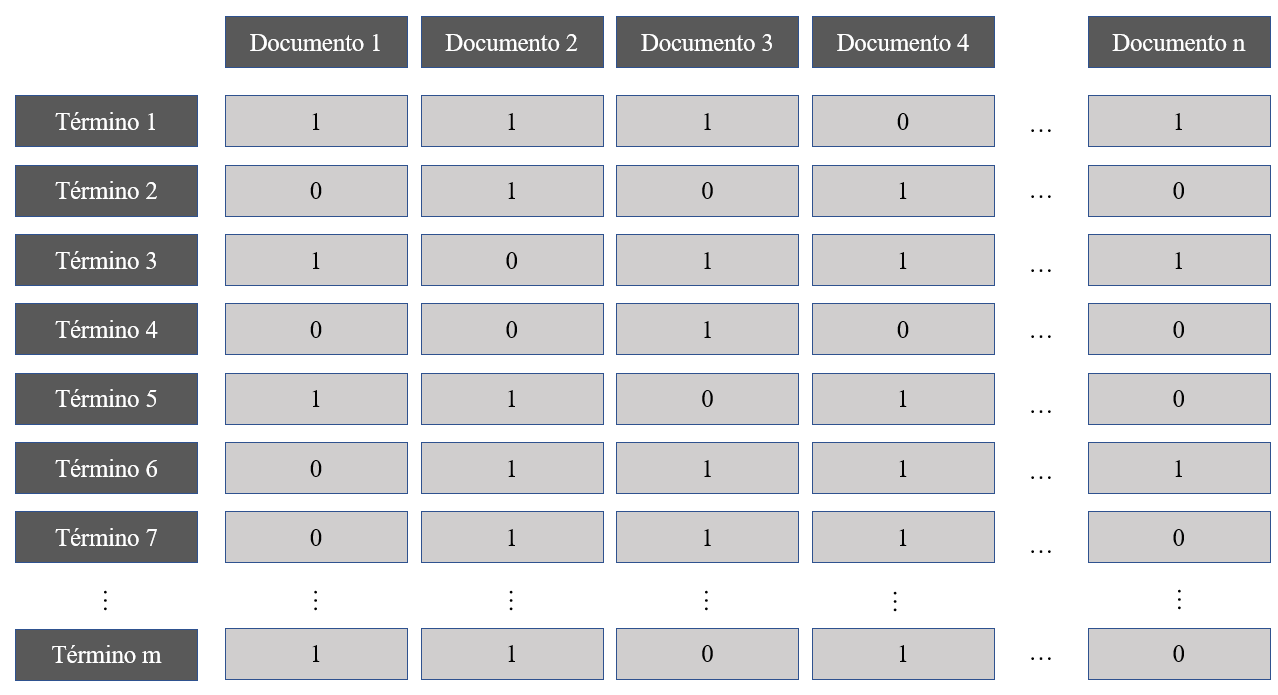
\includegraphics[scale=0.5]{doc/images/BS/b_matrix.PNG}
    \caption{Matriz binaria ejemplo}
    \label{fig:b_matrix}
\end{figure}

Tras recibir la consulta (palabras claves que caracterizan la necesidad de información) se procede a construir un vector del tamaño del vocabulario que indica, al igual que la matriz, qué términos incluye la consulta, generando así un vector binario disperso. En la figura \ref{fig:b_query} se muestra cómo sería el vector de la consulta.\\

\begin{figure}[]
    \centering
    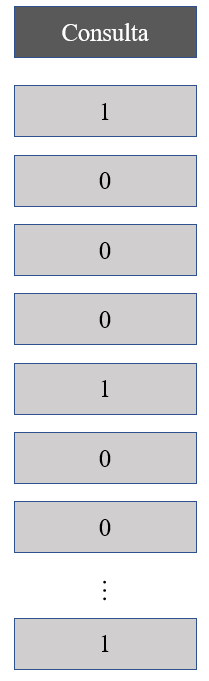
\includegraphics[scale = 0.5]{doc/images/BS/b_query.PNG}
    \caption{Vector binario de la consulta}
    \label{fig:b_query}
\end{figure}

En el caso específico del \textit{dataset} trabajado la matriz tiene dimensión de m filas, n columnas, dado que se tiene un vocabulario de m términos.\\

Con el fin de almacenar de manera eficiente una matriz de tamaño (mxn) se procede a utilizar el tipo de dato que menor espacio de memoria ocupa. Al momento de crear la matriz se indica el tipo de dato a utilizar, el cual corresponde a \url{numpy.bool\_}. Para guardar y abrir la matriz se utilizan las funciones estándar de numpy (\url{load} y \url{save}).\\

Ahora bien, una vez se tiene el vector que representa la consulta y la matriz que almacena toda la información de términos por documento, se utiliza una operación lógica que permita seleccionar los documentos que contienen uno o todos los términos consultados. En el primer caso se utiliza la operación lógica OR, lo cual indica que se extraerán los documentos que tienen al menos uno de los términos buscados; en caso contrario, se utiliza AND para obtener los documentos que tienen todos y cada uno de los términos buscados.\\

Como es de esperarse es poco común que un documento contenga exactamente todos los términos al igual que es muy probable que algún documento tenga al menos uno de los términos, ocasionando el fenómeno conocido como \textit{feast and famine}.